\documentclass{article}
\usepackage[utf8]{inputenc}
\usepackage[dutch]{varioref}
\usepackage[dutch]{babel}
\usepackage{pdfpages}

\title{Stageverslag}
\author{\mbox{Pieter-Jan} Robrecht}
\date{Maart 2016}
\usepackage{natbib}
\usepackage{graphicx}

\begin{document}

%\maketitle
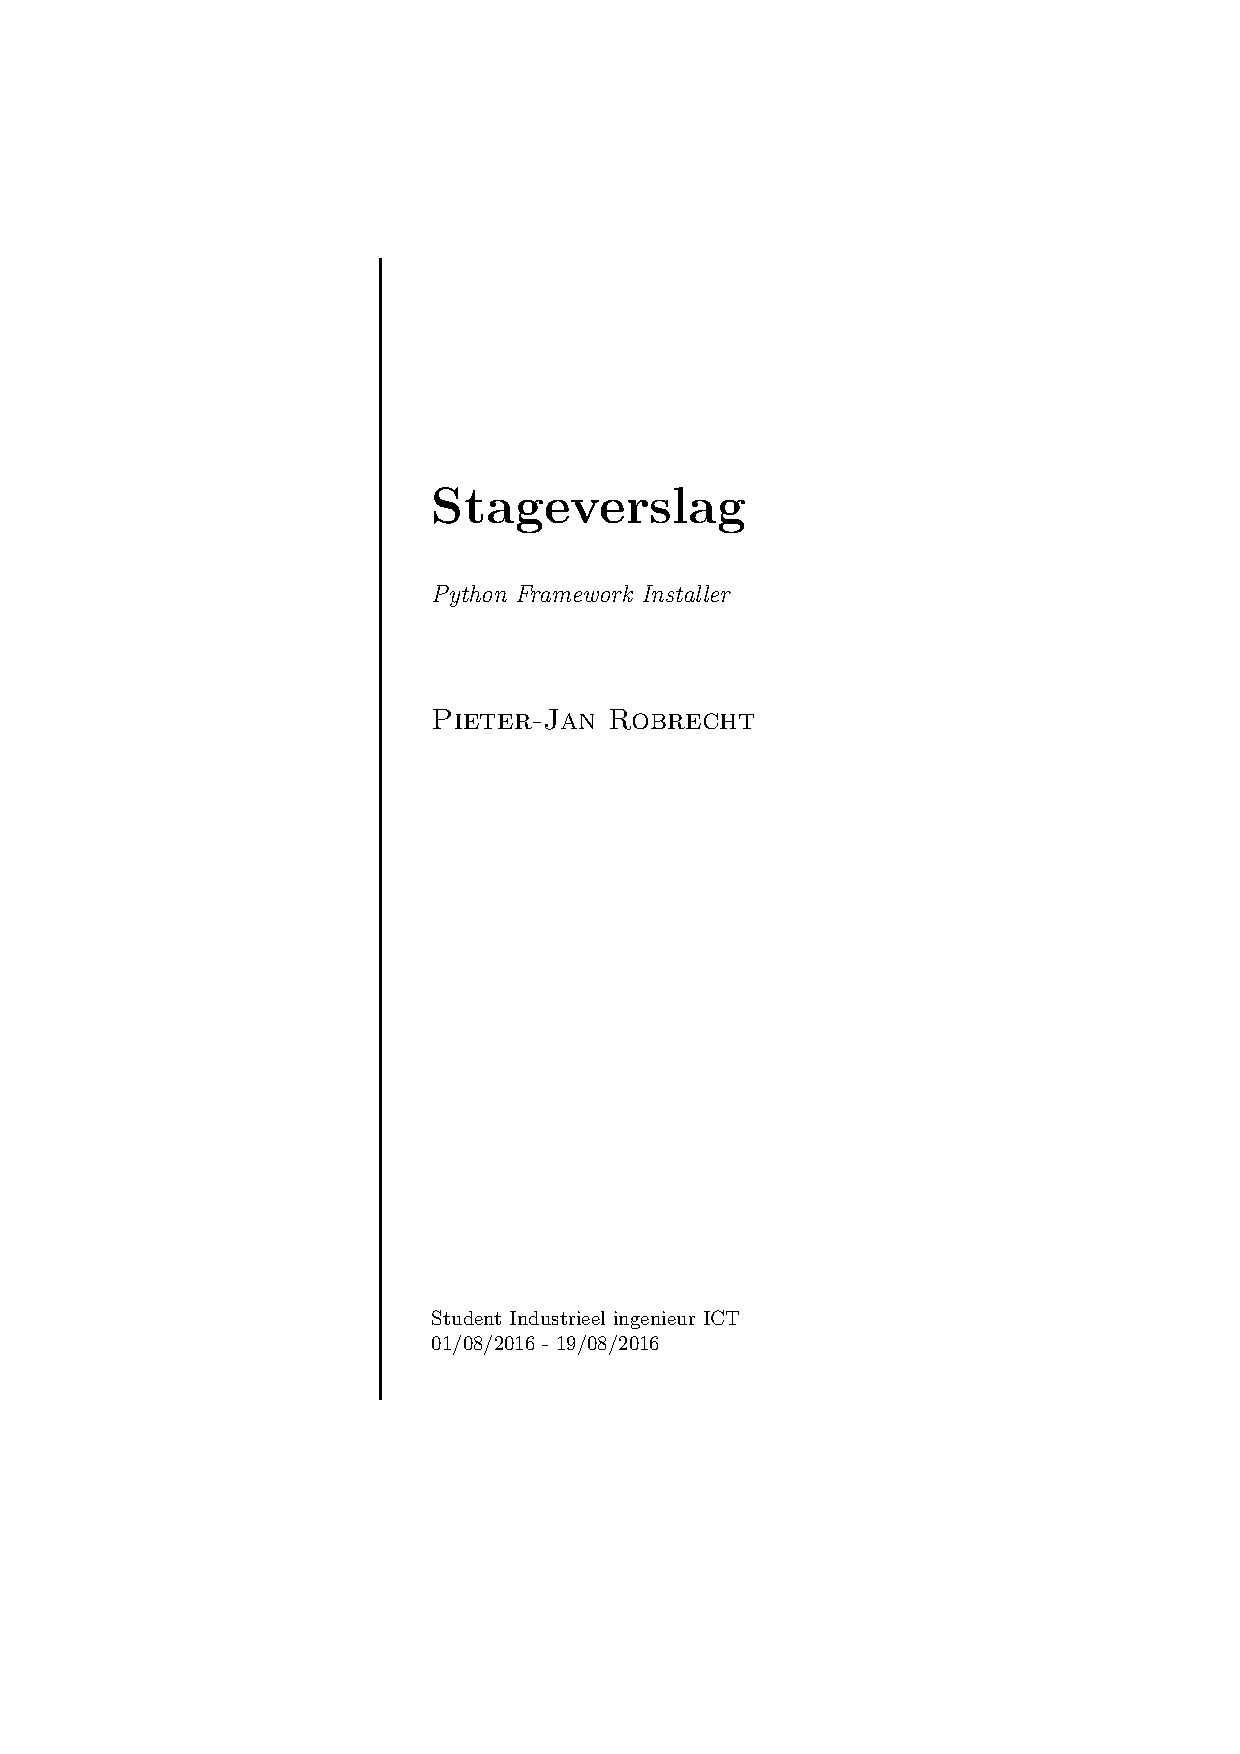
\includepdf{titel/titelstage.pdf}

%Volgende lijn is om de titelpagina geen paginanummer te geven
\clearpage
\setcounter{page}{1}

\tableofcontents
\clearpage

\section{Inleiding}
In het kader van mijn masterproef was het mogelijk om bij Televic Rail een stage te lopen tijdens de zomer. Gedurende deze stage zal ik mijn masterproef voorbereiden en onderzoek doen naar de verschillende mogelijkheden die er zijn voor het uitvoeren van mijn opdracht. 

\section{Analyse van het probleem}
Tijdens het bespreken van het probleem werd het al snel duidelijk dat er verschillende scenario's zijn waarin het framework gaat gebruikt moeten worden. Het framework zal gebruikt moeten worden als een standalone programma op een laptop of desktop maar het zal ook moeten draaien op de verschillende testtorens. Beide omgevingen zullen Windows gebruiken als besturingssysteem. Er zullen dus geen grote veranderingen moeten worden aangebracht in het maken van de installer aangezien beide omgevingen overweg kunnen met een .exe bestand. Uiteraard moet er rekening worden gehouden met de toekomst. Het framework zal in de nabije toekomst worden aangepast zodanig dat het mogelijks op een raspberry pi kan draaien. Dit zou wel voor verschillende problemen kunnen zorgen aangezien een raspberry pi een linux distributie zal gebruiken als zijn besturingssysteem. 

\section{Oplossingen}

\end{document}